\documentclass[10pt, aspectratio=1610]{beamer}
\usepackage{amsmath, amsfonts}
\usepackage{multirow}
\usepackage{array}
\usepackage{tikz}
\usepackage{pgfplots}
\usepackage{subfig}
\usepackage{threeparttable}
\usepackage{glossaries}
\usepackage{xcolor}
\usepackage[utf8]{inputenc}


\usepackage[ruled, vlined, linesnumbered]{algorithm2e}
\usepackage{hyperref}

\usepackage{roboto}

\usepackage{booktabs}
\usepackage{caption}
\usepackage{colortbl}

\usefonttheme{professionalfonts}

%% Set colors for the presentation
\definecolor{t1}{RGB}{239, 35, 60} %red
\definecolor{t2}{RGB}{43, 45, 66} %dark grey
\definecolor{t3}{RGB}{141, 153, 174} % gray

\setbeamercolor{title}{fg=t2}
\setbeamercolor{frametitle}{fg=t2}
\setbeamercolor{subtitle}{fg=t2}
\setbeamercolor{section in toc}{fg=t2}
\setbeamercolor{subsection in toc}{fg=t2}
\setbeamercolor{caption}{fg=t2}
\setbeamercolor{caption name}{fg=t2}
\setbeamercolor{item}{fg=t2}
\setbeamercolor{itemize item}{fg=t1}
\setbeamercolor{enumerate item}{fg=t2}

\setbeamertemplate{itemize item}[circle]
\setbeamertemplate{navigation symbols}{}
\setbeamertemplate{section in toc}[sections numbered]
\setbeamertemplate{subsection in toc}[subsections numbered]
\setbeamertemplate{caption}[numbered]
\setbeamertemplate{footline}[frame number]

\setbeamerfont{title}{series=\bfseries}
\setbeamerfont{section in toc}{series=\bfseries}
\setbeamerfont{frametitle}{series=\bfseries}
\setbeamerfont{caption name}{series=\bfseries}


\usetikzlibrary{arrows.meta}
\usetikzlibrary{datavisualization.formats.functions}

% \mode<presentation>
\title{Implementation of a Microgrid Energy Management System Considering 
E-Mobility, Uncertainties and Contingencies: A Multi-Objective Approach}

\author[Derian Tairo]{Derian Carlos Tairo Garcia \\
    \text{d255905@dac.unicamp.br}}
\date{\today}

\begin{document}
    
\begin{frame}
    \titlepage
\end{frame}

\begin{frame}
    \frametitle{Table of Contents}
    \tableofcontents
\end{frame}
% \logo{\includegraphics[height=1cm]{../Figures/unicamp_logo.png}}

\section{Introduction}

\begin{frame}
    \frametitle{Introduction}
    \begin{figure}
        \includegraphics[width = 0.8\textwidth]{../Figures/Microgrid_example.pdf}
    \end{figure}

\end{frame}



\begin{frame}
    \frametitle{Objectives}
    \begin{itemize}[<+->]
        \item Develop a multi-objective optimization model for the EMS. 
        \item Integrate a new window of EVs in the IoT-based EMS.
        \item Validate the EMS in a Hardware-in-the-Loop (HIL) environment.
    \end{itemize}
\end{frame}


\section{Methodology}
\subsection{Uncertainty and Contingency Sets}

\begin{frame}{Methodology}{Uncertainty and Contingency Sets}
    \begin{itemize}
        \item Uncertainties are addressed using multiple profiles for 
        solar generation and demand, 9 scenarios.
        \item Contingencies, reflecting all possible occurrences across the 
        24-hour period.
    \end{itemize}
\end{frame}

\begin{frame}{Methodology}{Uncertainty and Contingency Sets}
    \begin{figure}
        \begin{tikzpicture}[baseline]
            \begin{axis}[
            xlabel={Period time [h]},
            ylabel near ticks,
            xlabel near ticks,
            ylabel={Active Power [p.u.]},
            tick style = {line width = 0.5, color = lightgray, 
                major tick length=4pt,minor tick length=2pt,
                minor x tick num = 3, minor y tick num =1},
            tick label style = {font=\small, xtick distance=4, ytick distance=152,
                xticklabels={00:00, 00:00, 04:00, 08:00, 12:00, 16:00, 20:00},
                yticklabels={0,0,0.2,0.4,0.6,0.8,1.0}},
            legend style = {font=\footnotesize, at={(0.99,0.98)}, 
                legend cell align=left, line width=0.5pt, draw=lightgray},
            % legend entries={High PV, Medium PV, Low PV, High load, Medium load, Low load},
            ymin=0, ymax=760,
            xmin=0, xmax=23,
            width=12cm,
            height=7.5cm,
            axis line style = {lightgray, line width = 0.5pt},
            cycle multi list={
            black, gray\nextlist
            linestyles
            }
            ]
            \addplot  table 
                [col sep=comma, x=h, y=pv_h] {../Data/pv_pd.dat};
            \addlegendentry[]{High PV}
            \addplot  table 
                [col sep=comma, x=h, y=pd_h] {../Data/pv_pd.dat}; 
            \addlegendentry{High load}     
            \only<2->{\addplot  table 
                [col sep=comma, x=h, y=pd_m] {../Data/pv_pd.dat};
                \addlegendentry{Medium load}}
            \only<3->{\addplot  table 
                [col sep=comma, x=h, y=pd_l] {../Data/pv_pd.dat};
                \addlegendentry{Low load}}
        
            \only<4->{\addplot  table 
                [col sep=comma, x=h, y=pv_m] {../Data/pv_pd.dat};
                \addlegendentry{Medium PV}}
            \only<5->{\addplot  table 
                [col sep=comma, x=h, y=pv_l] {../Data/pv_pd.dat};
                \addlegendentry{Low PV}}
            \end{axis}
        \end{tikzpicture} 
    \caption{Scenarios for solar generation and demand.}
    \end{figure}

\end{frame}

\begin{frame}{Methodology}{Uncertainty and Contingency Sets}
    \begin{figure}
        \begin{tikzpicture}[xscale=1.5, yscale=1, baseline]
            % \draw[help lines] (0,0) grid (5,5);
        \only<1>{
            %grid lines
            \draw [lightgray, dotted, line width=1, <->][Triangle-Triangle] 
                    (0,4.5) -- (5,4.5);
        
            % body
            \draw [fill=lightgray] (0,4) rectangle (1,5);
                \draw [black, line width=0.5, <->][Triangle-Triangle] 
                    (0,5.1) -- (1,5.1);
                \node [above] at (0.5,5.1) {$t_{1} + \Delta t_{c}$};
                    \node at (0.5,4.5) {$\mathcal{C}_{1}$};
            %axis lines        
            \draw [lightgray, dotted, line width=0.5]  (0,0) -- (0,5);
            \draw [lightgray, dotted, line width=0.5]  (5,0) -- (5,5);
            \draw [lightgray, line width=1 ] (0,0) -- (5,0);
            %\draw [black, line width=1 ] (0,5.5) -- (5,5.5);
        }

        \only<2>{
            \draw [lightgray, dotted, line width=1, <->][Triangle-Triangle] 
                    (0,3.5) -- (5,3.5);

            \draw [lightgray, dotted, line width=0.5] 
                    (0.5,0) -- (0.5,3);

            \draw [lightgray, dotted, line width=0.5] 
                    (1.5,0) -- (1.5,4);

            % body
            \draw [fill=lightgray] (0.5,3) rectangle (1.5,4);
                \draw [black, line width=0.5, <->][Triangle-Triangle] 
                (0.5,4.1) -- (1.5,4.1);
                \node [above] at (1,4.2) {$t_{2} + \Delta t_{c}$};
                    \node at (1,3.5) {$\mathcal{C}_{2}$};

            %axis lines        
            \draw [lightgray, dotted, line width=0.5]  (0,0) -- (0,5);
            \draw [lightgray, dotted, line width=0.5]  (5,0) -- (5,5);
            \draw [lightgray, line width=1 ] (0,0) -- (5,0);
        }

        \only<3>{      
                    %grid lines
            \draw [lightgray, dotted, line width=1, <->][Triangle-Triangle] 
                    (0,4.5) -- (5,4.5);
            \draw [lightgray, dotted, line width=1, <->][Triangle-Triangle] 
                    (0,3.5) -- (5,3.5);
            \draw [lightgray, dotted, line width=1, <->][Triangle-Triangle] 
                    (0,2.5) -- (5,2.5);
            \draw [lightgray, dotted, line width=1, <->][Triangle-Triangle] 
                    (0,0.5) -- (5,0.5);
        
            \draw [lightgray, dotted, line width=0.5] 
                    (0.5,0) -- (0.5,3);
            \draw [lightgray, dotted, line width=0.5] 
                    (1,0) -- (1,2);
            \draw [lightgray, dotted, line width=0.5] 
                    (1.5,0) -- (1.5,2);
            \draw [lightgray, dotted, line width=0.5] 
                    (2,0) -- (2,2);
        
            \node[below] at (3,2) {$\ddots$};
        
            % body
            \draw [fill=lightgray] (0,4) rectangle (1,5);
                \draw [black, line width=0.5, <->][Triangle-Triangle] 
                    (0,5.1) -- (1,5.1);
                \node [above] at (0.5,5.1) {$t_{1} + \Delta t_{c}$};
                    \node at (0.5,4.5) {$\mathcal{C}_{1}$};
        
            \draw [fill=lightgray] (0.5,3) rectangle (1.5,4);
                    \node at (1,3.5) {$\mathcal{C}_{2}$};
        
            \draw [fill=lightgray] (1,2) rectangle (2,3);

                    \node at (1.5,2.5) {$\mathcal{C}_{3}$};

        
            \draw [fill=lightgray] (4,0) rectangle (5,1);
                \draw [black, line width=0.5, <->] [Triangle-Triangle] 
                    (4,1.1) -- (5,1.1);
                \node [above] at (4.5,1.1) {$t_{24} + \Delta t_{c}$};
                    \node at (4.5,0.5) {$\mathcal{C}_{24}$};
        
            %axis lines        
            \draw [lightgray, dotted, line width=0.5]  (0,0) -- (0,5);
            \draw [lightgray, dotted, line width=0.5]  (5,0) -- (5,5);
            \draw [lightgray, line width=1 ] (0,0) -- (5,0);

        }
            % x labels
            \node[below] at (0,0) {$t_1$};
            \node[below] at (0.5,0) {$t_2$};
            \node[below] at (1,0) {$t_3$};
            \node[below] at (1.5,0) {$t_4$};
            \node[below] at (2,0) {$t_5$};
            \node[below] at (4,0) {$t_{22}$};
            \node[below] at (4.5,0) {$t_{23}$};
            \node[below] at (5,0) {$t_{24}$};
            \node[below] at (3,-0.1) {$\dotsc$};
        
            \node[below] at (2.5,-0.5) {$\text{Period time [h]}$};    
        \end{tikzpicture}
        \caption{Set of contingencies}
    \end{figure}
\end{frame}

\subsection{Mathematical Model for the EMS}

\begin{frame}{Methodology}{Mathematical Model for the EMS}
\begin{itemize}[<+->]
    \item Objective function 1
    \begin{multline}\label{obj_1}
        {f_{costs}} = \min \Delta t \sum_{s \in \mathcal{S}} 
            \Biggl\{ \mathit{Prob}_{s} \cdot \Bigg[
                \sum_{i \in \mathcal{N}} 
                \sum_{f \in \mathcal{F}} 
                \sum_{t \in \mathcal{T}} 
                \sum_{c \in \mathcal{C}} 
        \alpha_{t}^{\text{S}} P_{i,f,t,c,s}^{\text{PCC}} + \\
            \sum_{n \in \mathcal{G}} 
            \sum_{t \in \mathcal{T}} 
            \sum_{c \in \mathcal{C}} 
        \Big(P^{\text{G}}_{n,t,c,s} \cdot \alpha_{n}^{\text{G}} \cdot \mu_{n,t,c,s} \Big) + \\
            \sum_{i \in \mathit{N}} 
            \sum_{f \in \mathit{F}}
            \sum_{t \in \mathit{T}}
            \sum_{c \in \mathit{C}} \alpha^{\text{C}} P_{i,f,t}^{\text{D}} 
                (1 - x_{i,f,t,c}) \Bigg] \Biggr\} 
        \end{multline}

    \item Objective function 2
    \begin{equation}\label{obj_2}
            {f_{ens}} = \min \sum_{\forall r,t | t=t_{d}} 
                \left( \overline{{E}_{r}^{\mathrm{EV}}} - {E}_{r,t}^{\mathrm{EV}} \right)
    \end{equation}
\end{itemize}

\end{frame}

\begin{frame}{Methodology}{Mathematical Model for the EMS}
    \textbf{Subject to:} 

    \begin{itemize}%[<+->]
        \item Constraints related to the operation of three-phase distribution 
        systems
        \item Constraints related to genset operation
        \item Constraints related to islanded operation
        \item Constraints related to BESS
        \item Constraints related to EVs
    \end{itemize}
\end{frame}

\subsection{Multi-objective Optimization Problem}

\begin{frame}{Methodology}{Multi-objective Optimization Problem}
    \textbf{To solve MOOP, we employ the $\epsilon$-constraint method}
\end{frame}

\begin{frame}{Methodology}{Multi-objective Optimization Problem}
    \begin{equation}
        \left.
        \begin{aligned}
        \textbf{minimize} &\quad \text{$f_{costs}$}\\
        \textbf{subject to}&\quad \text{$f_{ens}$} \leq \text{$\varepsilon_{p}$},\\
        &\text{Operation of three-phase distribution 
        systems}\\
        &\text{Islanded operation}\\
        &\text{Genset operation}\\
        &\text{BESS} \\
        &\text{EVs}
        \end{aligned}
        \right\}
        \label{final_equation}
    \end{equation}
\end{frame}

\section{EMS software architecture}
\subsection{Backend and Frontend} 

\begin{frame}{EMS software architecture}
    \begin{figure}  
    \only<1>{\includegraphics[width=0.95\textwidth]
    {../Figures/ems_architecture_1.pdf}}
    \only<2>{\includegraphics[width=0.95\textwidth]
    {../Figures/ems_architecture_2.pdf}}
    \only<3>{\includegraphics[width=0.95\textwidth]
    {../Figures/ems_architecture_3.pdf}}
    \only<4>{\includegraphics[width=0.95\textwidth]
    {../Figures/ems_architecture.pdf}}
    \caption{IoT-based for microgrids software architecture.}
    \end{figure}
\end{frame}

\begin{frame}{EMS software architecture}
    \begin{figure}
        \includegraphics[width=0.98\textwidth]{../Figures/EMS/dashboard.jpg}
        \caption{Frontend of GUI EMS.}
    \end{figure}
\end{frame}

\begin{frame}{EMS software architecture}
    \begin{figure}
        \includegraphics[width=0.98\textwidth]{../Figures/EMS/EVs.png}
        \caption{Frontend of GUI EMS - EVs tab.}
    \end{figure}
\end{frame}

\section{Case study}

\begin{frame}{Case study: CAMPUSGRID microgrid}
    \begin{figure}
        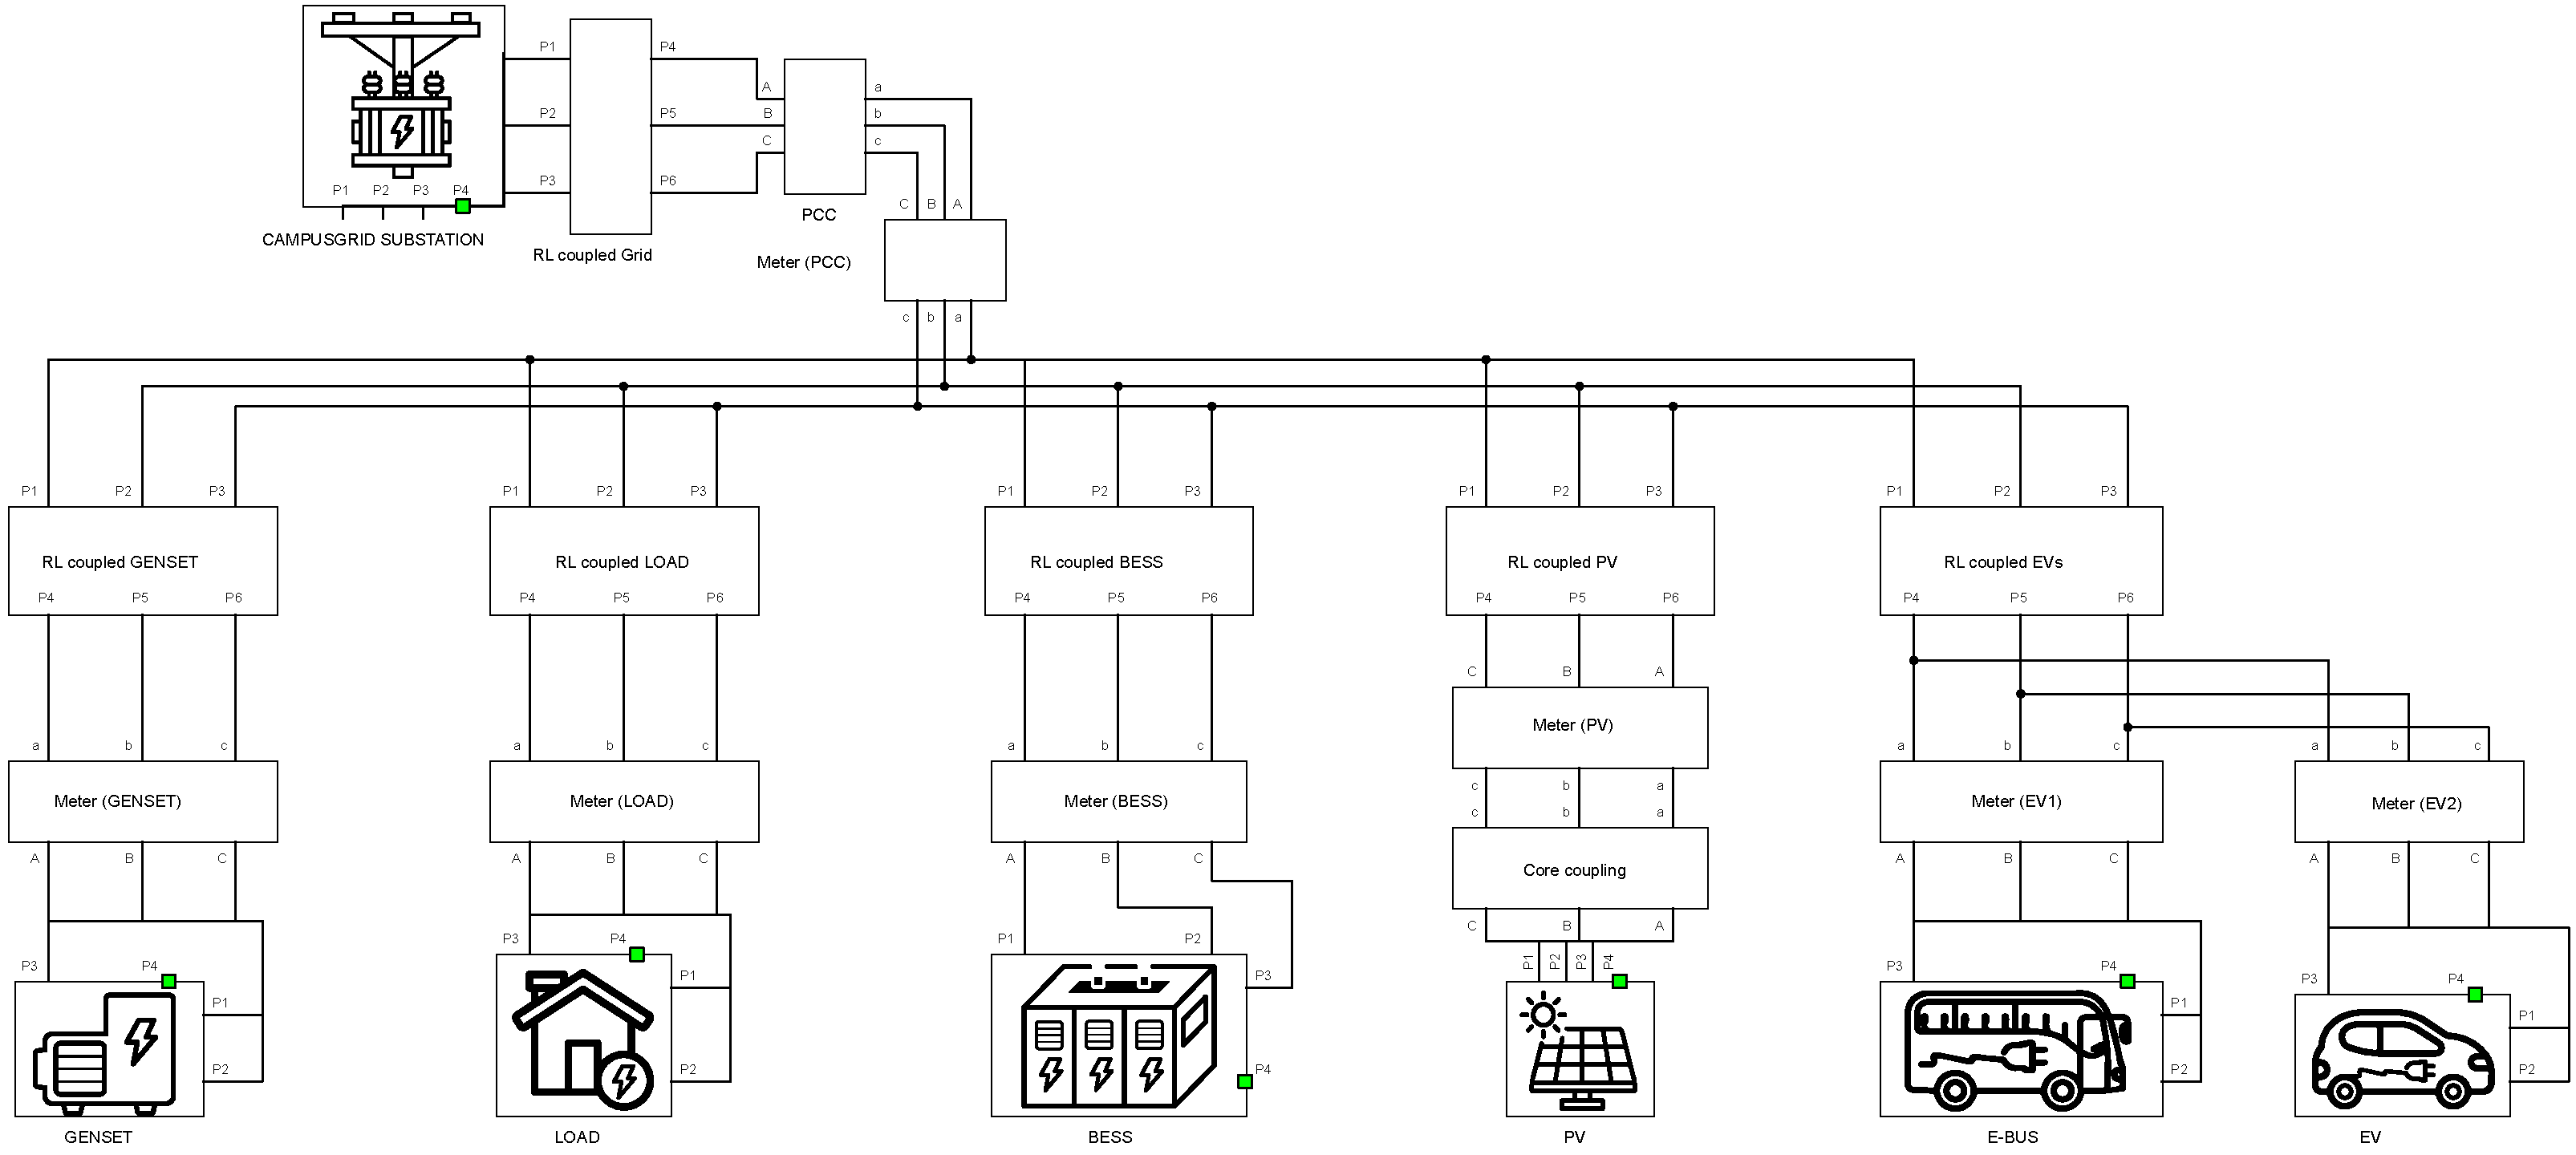
\includegraphics[width=0.98\textwidth]{../Figures/schematic_HIL.pdf}
        \caption{Microgrid CAMPUSGRID schematic in Typhoon HIL 604.}
    \end{figure}
\end{frame}

% \begin{frame}
%     \begin{table}[!htb]
%     \caption{Microgrid parameters.}
%     \vspace{-9pt}
%         \begin{center}
%             \begin{threeparttable}
%                 \begin{tabular}{cccc}
%                     \hline
%                     Device & Parameter & Magnitude & Unit\\
%                     \hline
%                     \multirow{7}{*}{Grid}
%                     &$\overline{{V}_{i}}$, $\underline{{V}_{i}}$ 
%                     &\multicolumn{1}{l}{1.05 \quad 0.95} & [kVA]\\
%                     &${S}^{\text{sub}}$ & 2375 & [\%]\\
%                     &$\overline{{I}^{\text{PCC}}}$ & 1000 & [A]\\
%                     &${V}^{nom}$ & 11.9 & [kW]\\
%                 &${P}^{\text{D}}_{i}$ & 371 & [kW]\\
%                 &${Q}^{\text{D}}_{i}$ & 260 & [kW]\\
%                 &${P}^{\text{PV}}_{i}$ & 736 & [kWp]\\
                
%                 \hline
                
%                 \multirow{3}{*}{Genset}
%                 &$\overline{{P}^{\text{G}}_{n}}$, $\underline{{P}^{\text{G}}_{n}}$ 
%                 &\multicolumn{1}{l}{150 \quad 0} & [kW]\\
%                 &$\overline{{Q}^{\text{G}}_{n}}$ , $\underline{{Q}^{\text{G}}_{n}}$
%                 &\multicolumn{1}{l}{150 \quad -150}&[kVAr]\\
%                 &$\alpha_{n}^{\text{G}}$ &30&[m.u.]\\
%                 \hline
%                 \multirow{4}{*}{BESS}
%                 &$\overline{{P}^{\text{B}}_{m}}$, $\underline{{E}^{\text{B}}_{m}}$ 
%                 &\multicolumn{1}{l}{1275 \quad 260} & [kWh]\\
%                 &$\eta^{\text{B}}$ &95&[\%]\\
%                 &${E}^{\text{B}_{\circ}}_{m}$ &260&[kWh]\\
%                 &$\overline{{P}^{\text{B}}_{m}}$ &1000&[kW]\\
%                 \hline
%                 \multirow{4}{*}{EV}
%                 &$\overline{{E}^{\text{EV}}_{r}}$, $\underline{{E}^{\text{EV}}_{r}}$ 
%                 &\multicolumn{1}{l}{324 \quad 64.8} & [kWh]\\
%                 &$\eta^{\text{EV}}$ & 95 & [\%]\\
%                 &${E}^{\text{EV}_{\circ}}_{r}$ & 64.8 & [kWh]\\
%                 &$\overline{{P}^{\text{EV}}_{r}}$ & 80 & [kW]\\
%                 \hline
%             \end{tabular}
%             \end{threeparttable}
%         \end{center}
%     \end{table}
% \end{frame}

\begin{frame}{Case study}
    \begin{itemize}
        \item Case I: Without contingencies.
        \item Case II: Contingency at 16:00 hours.
        \item Case III: Contingency at 08:00 hours. 
        \item Case IV: Without contingencies, including EV.
        \item Case V: Contingency at 16:00 hours with EV.
        \item Case VI: Contingency at 08:00 hours with  EV. 
        \item Case VII: Contingencies at 08:00 and 16:00 hours with EVs.
    \end{itemize}
\end{frame}


\section{Results}
\subsection{Multi-objective Optimization Analysis}

\begin{frame}
    \frametitle<2>{Test and Results}
    \framesubtitle<2>{Multi-objective Optimization Analysis}
    
    \only<1>{
        \textbf{Remembering the MOOP:}
        \textbf{}
        \begin{equation*}
            \left.
            \begin{aligned}
            \textbf{minimize} &\quad \text{$f_{costs}$}\\
            \textbf{subject to}&\quad \text{$f_{ens}$} \leq \text{$\varepsilon_{p}$},\\
            &\text{Operation of three-phase distribution 
            systems}\\
            &\text{Islanded operation}\\
            &\text{Genset operation}\\
            &\text{BESS} \\
            &\text{EVs}
            \end{aligned}
            \right\}
            (3)
        \end{equation*}
        }
    \only<2>{
        \begin{algorithm}[H]
        \caption{$\varepsilon$-Constraint Method for MOOP}
        \label{alg:e_constraint_method}
        \SetAlgoLined
        \KwData{Parameters of the MOOP, including scenarios and contingencies}
        \KwResult{Pareto front}
        \BlankLine
        \textbf{Initialize:} Set of $\varepsilon_{p}$ values\;
        \For{each $\varepsilon_{p}$ value in the set}{
                \textbf{Solve:} \eqref{final_equation}\;
                \textbf{Store:} Non-dominated solutions\;
            }
        \BlankLine
        \textbf{Generate} Pareto front\;
        \textbf{Compute:} The centroid of the Pareto front\;
    \end{algorithm}
    }
\end{frame}

\begin{frame}{Tests and Results}
\framesubtitle{Multi-objective Optimization Analysis}
    \begin{figure}
        \only<1>{
            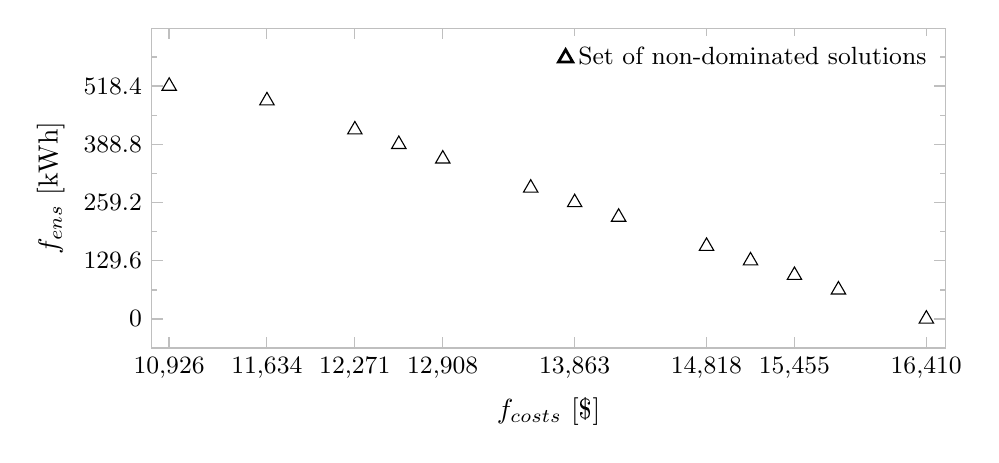
\begin{tikzpicture}
            \begin{axis}[
                width=0.5\textwidth,
                height = 0.8\textwidth,
                y post scale = 0.5,
                x post scale = 2.25,
                xlabel={$f_{costs}$ [\$]},
                xlabel near ticks,
                ylabel={$f_{ens}$ [kWh]},
                ylabel near ticks,
                tick style = {line width = 0.5, color = lightgray, 
                    major tick length=4pt,minor tick length=2pt, 
                    minor y tick num =1, xtick = {10926, 11634, 12271,
                    12908, 13863, 14818, 15455, 16410}
                    },
                tick label style = {font=\small, ytick distance=129.6
                    },
                xtick align = {inside},
                ytick align = {inside},
                legend style = {font=\small, at={(0.995,0.98)},    
                    anchor= north east, legend cell align=center, line width=1pt, 
                    draw = none, legend columns = 2},
                ymax=647,
                xmin=10800, xmax=16550,
                axis line style = {line width = 0.5pt, lightgray},
                scaled ticks=false
                ]
            
            % Set of non-dominated solutions 
            \addplot[mark = triangle, only marks, mark size = 3pt,
            black] 
            coordinates {
                (10926.93, 518.4)
                (11634.98, 486.0)
                % (11953.37, 453.6)
                (12271.76, 421.2)
                (12590.16, 388.8)
                (12908.55, 356.4)
                % (13226.95, 324.0)
                (13545.34, 291.6)
                (13863.73, 259.2)
                (14182.13, 226.8)
                % (14110.87, 194.4)
                (14818.92, 162.0)
                (15137.31, 129.6)
                (15455.70, 97.2)
                % (15702.84, 32.4)
                (15774.10, 64.8)
                (16410.89, 0)               
                };
            \addlegendentry{Set of non-dominated solutions}
    
            \end{axis}
        \end{tikzpicture}
        \caption{Pareto front}
        }
        \only<2>{
            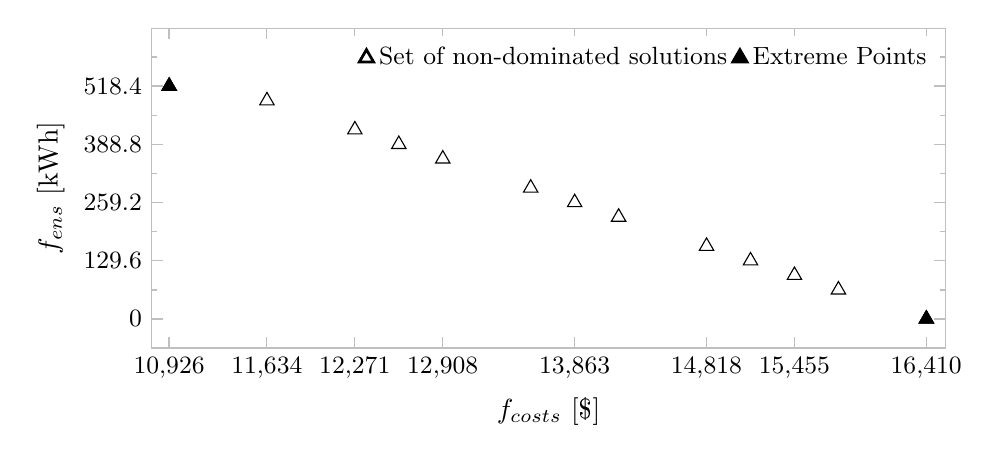
\begin{tikzpicture}
            \begin{axis}[
                width=0.5\textwidth,
                height = 0.8\textwidth,
                y post scale = 0.5,
                x post scale = 2.25,
                xlabel={$f_{costs}$ [\$]},
                xlabel near ticks,
                ylabel={$f_{ens}$ [kWh]},
                ylabel near ticks,
                tick style = {line width = 0.5, color = lightgray, 
                    major tick length=4pt,minor tick length=2pt, 
                    minor y tick num =1, xtick = {10926, 11634, 12271,
                    12908, 13863, 14818, 15455, 16410}
                    },
                tick label style = {font=\small, ytick distance=129.6
                    },
                xtick align = {inside},
                ytick align = {inside},
                legend style = {font=\small, at={(0.995,0.98)},    
                    anchor= north east, legend cell align=center, line width=1pt, 
                    draw = none, legend columns = 2},
                ymax=647,
                xmin=10800, xmax=16550,
                axis line style = {line width = 0.5pt, lightgray},
                scaled ticks=false
                ]
            
            % Set of non-dominated solutions 
            \addplot[mark = triangle, only marks, mark size = 3pt,
            black] 
            coordinates {
                (10926.93, 518.4)
                (11634.98, 486.0)
                % (11953.37, 453.6)
                (12271.76, 421.2)
                (12590.16, 388.8)
                (12908.55, 356.4)
                % (13226.95, 324.0)
                (13545.34, 291.6)
                (13863.73, 259.2)
                (14182.13, 226.8)
                % (14110.87, 194.4)
                (14818.92, 162.0)
                (15137.31, 129.6)
                (15455.70, 97.2)
                % (15702.84, 32.4)
                (15774.10, 64.8)
                (16410.89, 0)               
                };
            \addlegendentry{Set of non-dominated solutions}
            
            % Centroid
            \addplot [mark size = 3pt, only marks, mark = triangle*]
                coordinates {
                (10926.93, 518.4)
                (16410.89, 0)               
                };
            \addlegendentry{Extreme Points}  
            \end{axis}
        \end{tikzpicture}
        \caption{Pareto front}
        }
        \only<3>{
            \tikzstyle{every pin}=[
                fill=white,
                draw=gray,
                font=\footnotesize]
            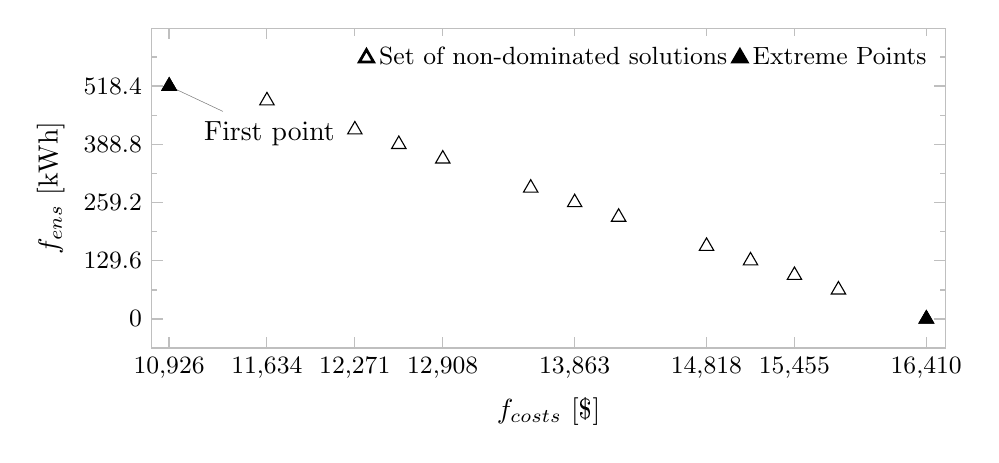
\begin{tikzpicture}
            \begin{axis}[
                width=0.5\textwidth,
                height = 0.8\textwidth,
                y post scale = 0.5,
                x post scale = 2.25,
                xlabel={$f_{costs}$ [\$]},
                xlabel near ticks,
                ylabel={$f_{ens}$ [kWh]},
                ylabel near ticks,
                tick style = {line width = 0.5, color = lightgray, 
                    major tick length=4pt,minor tick length=2pt, 
                    minor y tick num =1, xtick = {10926, 11634, 12271,
                    12908, 13863, 14818, 15455, 16410}
                    },
                tick label style = {font=\small, ytick distance=129.6
                    },
                xtick align = {inside},
                ytick align = {inside},
                legend style = {font=\small, at={(0.995,0.98)},    
                    anchor= north east, legend cell align=center, line width=1pt, 
                    draw = none, legend columns = 2},
                ymax=647,
                xmin=10800, xmax=16550,
                axis line style = {line width = 0.5pt, lightgray},
                scaled ticks=false
                ]
            
            % Set of non-dominated solutions 
            \addplot[mark = triangle, only marks, mark size = 3pt,
            black] 
            coordinates {
                (10926.93, 518.4)
                (11634.98, 486.0)
                % (11953.37, 453.6)
                (12271.76, 421.2)
                (12590.16, 388.8)
                (12908.55, 356.4)
                % (13226.95, 324.0)
                (13545.34, 291.6)
                (13863.73, 259.2)
                (14182.13, 226.8)
                % (14110.87, 194.4)
                (14818.92, 162.0)
                (15137.31, 129.6)
                (15455.70, 97.2)
                % (15702.84, 32.4)
                (15774.10, 64.8)
                (16410.89, 0)               
                };
            \addlegendentry{Set of non-dominated solutions}
            
            % Centroid
            \addplot [mark size = 3pt, only marks, mark = triangle*]
                coordinates {
                (10926.93, 518.4)
                (16410.89, 0)               
                };
            \addlegendentry{Extreme Points}
            \node [coordinate, pin=below right:{First point}] at
                (axis cs: 10926.93, 518.4 ) {};
    
            \end{axis}
        \end{tikzpicture}
        \caption{Pareto front}
        }
        \only<4>{%Dispatch of the BESS and EVs
            \begin{tikzpicture}
                \begin{axis}[ybar stacked,
                    xlabel={Period time [h]},
                    ylabel={Active power [kW]},
                    ylabel near ticks,
                    xlabel near ticks,
                    bar width=4pt,
                    tick style = {line width = 0.5, color = lightgray, 
                        major tick length=4pt,minor tick length=2pt,
                        minor x tick num = 3, minor y tick num =2},
                    tick label style = {font=\small, xtick distance=4, ytick distance=200,
                        xticklabels={01:00, 01:00, 04:00, 08:00, 12:00, 16:00, 20:00 }},
                    legend style = {font=\footnotesize, at={(0.99,0.98)}, 
                        legend cell align=left, line width=0.5pt, draw=lightgray},
                    legend entries={BESS,EV 1,EV 2},
                    ymin=-350, ymax=300,
                    xmin=0, xmax=25,
                    axis line style = {lightgray, line width = 0.5pt},
                    cycle multi list={
                    lightgray, darkgray, color=t1\nextlist
                    fill
                    }
                    ]
            
                    \addplot table 
                    [col sep=comma, x = h,y=P_BESS] {../Data/second_point.dat};
                    \addplot table
                    [col sep=comma, x = h, y=P_EV_1] {../Data/second_point.dat};
                    \addplot table
                    [col sep=comma, x = h,y=P_EV_2] {../Data/second_point.dat};
            
                \end{axis}
            \end{tikzpicture}
        }
        \only<5>{
            \tikzstyle{every pin}=[
                fill=white,
                draw=gray,
                font=\footnotesize]
            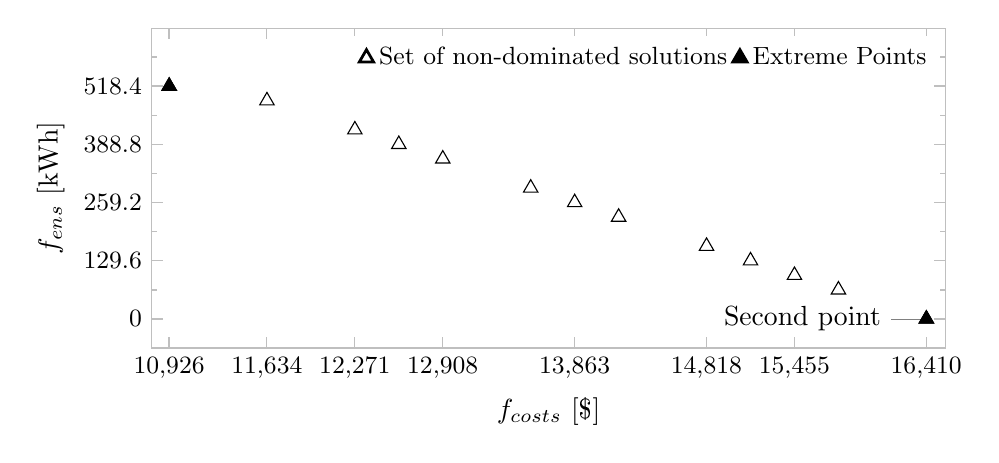
\begin{tikzpicture}
            \begin{axis}[
                width=0.5\textwidth,
                height = 0.8\textwidth,
                y post scale = 0.5,
                x post scale = 2.25,
                xlabel={$f_{costs}$ [\$]},
                xlabel near ticks,
                ylabel={$f_{ens}$ [kWh]},
                ylabel near ticks,
                tick style = {line width = 0.5, color = lightgray, 
                    major tick length=4pt,minor tick length=2pt, 
                    minor y tick num =1, xtick = {10926, 11634, 12271,
                    12908, 13863, 14818, 15455, 16410}
                    },
                tick label style = {font=\small, ytick distance=129.6
                    },
                xtick align = {inside},
                ytick align = {inside},
                legend style = {font=\small, at={(0.995,0.98)},    
                    anchor= north east, legend cell align=center, line width=1pt, 
                    draw = none, legend columns = 2},
                ymax=647,
                xmin=10800, xmax=16550,
                axis line style = {line width = 0.5pt, lightgray},
                scaled ticks=false
                ]
            
            % Set of non-dominated solutions 
            \addplot[mark = triangle, only marks, mark size = 3pt,
            black] 
            coordinates {
                (10926.93, 518.4)
                (11634.98, 486.0)
                % (11953.37, 453.6)
                (12271.76, 421.2)
                (12590.16, 388.8)
                (12908.55, 356.4)
                % (13226.95, 324.0)
                (13545.34, 291.6)
                (13863.73, 259.2)
                (14182.13, 226.8)
                % (14110.87, 194.4)
                (14818.92, 162.0)
                (15137.31, 129.6)
                (15455.70, 97.2)
                % (15702.84, 32.4)
                (15774.10, 64.8)
                (16410.89, 0)               
                };
            \addlegendentry{Set of non-dominated solutions}
            
            % Centroid
            \addplot [mark size = 3pt, only marks, mark = triangle*]
                coordinates {
                (10926.93, 518.4)
                (16410.89, 0)               
                };
            \addlegendentry{Extreme Points}
            \node [coordinate, pin= left:{Second point}] at
                (axis cs: 16410.89, 0 ) {};
    
            \end{axis}
        \end{tikzpicture}
        \caption{Pareto front}
        }
        \only<6>{
            \begin{tikzpicture}
                \begin{axis}[ybar stacked,
                    xlabel={Period time [h]},
                    ylabel={Active power [kW]},
                    ylabel near ticks,
                    xlabel near ticks,
                    bar width=4pt,
                    tick style = {line width = 0.5, color = lightgray, 
                        major tick length=4pt,minor tick length=2pt,
                        minor x tick num = 3, minor y tick num =1},
                    tick label style = {font=\small, xtick distance=4, ytick distance=200,
                        xticklabels={01:00, 01:00, 04:00, 08:00, 12:00, 16:00, 20:00 }},
                    legend style = {font=\footnotesize, at={(0.99,0.98)}, 
                        legend cell align=left, line width=0.5pt, draw=lightgray},
                    legend entries={BESS,EV 1,EV 2},
                    ymin=-350, ymax=850,
                    xmin=0, xmax=25,
                    axis line style = {lightgray, line width = 0.5pt},
                    cycle multi list={
                    lightgray, darkgray, color=t1\nextlist
                    fill
                    }
                    ]
            
                    \addplot table 
                    [col sep=comma, x = h, y=P_BESS] {../Data/firs_point.dat};
                    \addplot table
                    [col sep=comma, x = h, y=P_EV_1] {../Data/firs_point.dat};
                    \addplot table
                    [col sep=comma, x = h, y=P_EV_2] {../Data/firs_point.dat};
                    
                \end{axis}
            \end{tikzpicture}
        }
        \only<7>{
            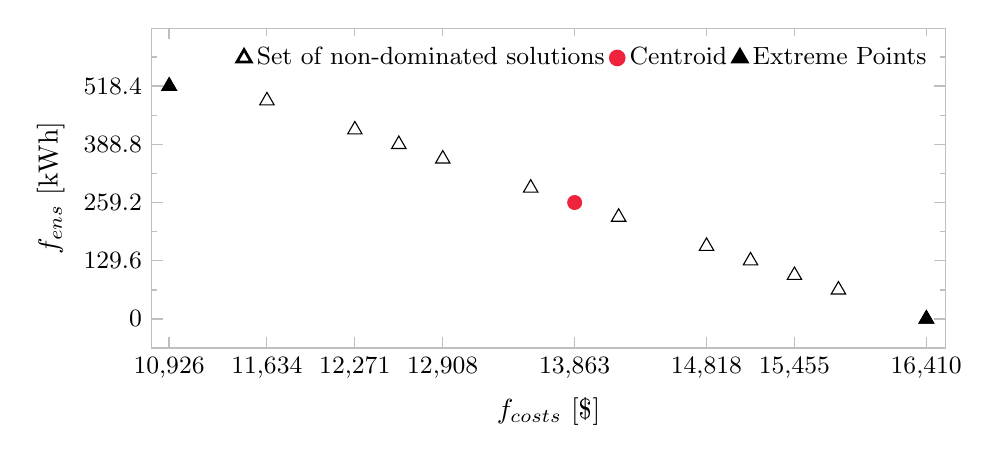
\begin{tikzpicture}
            \begin{axis}[
                width=0.5\textwidth,
                height = 0.8\textwidth,
                y post scale = 0.5,
                x post scale = 2.25,
                xlabel={$f_{costs}$ [\$]},
                xlabel near ticks,
                ylabel={$f_{ens}$ [kWh]},
                ylabel near ticks,
                tick style = {line width = 0.5, color = lightgray, 
                    major tick length=4pt,minor tick length=2pt, 
                    minor y tick num =1, xtick = {10926, 11634, 12271,
                    12908, 13863, 14818, 15455, 16410}
                    },
                tick label style = {font=\small, ytick distance=129.6
                    },
                xtick align = {inside},
                ytick align = {inside},
                legend style = {font=\small, at={(0.995,0.98)},    
                    anchor= north east, legend cell align=center, line width=1pt, 
                    draw = none, legend columns = 3},
                ymax=647,
                xmin=10800, xmax=16550,
                axis line style = {line width = 0.5pt, lightgray},
                scaled ticks=false
                ]
            
            % Set of non-dominated solutions 
            \addplot[mark = triangle, only marks, mark size = 3pt,
            black] 
            coordinates {
                (10926.93, 518.4)
                (11634.98, 486.0)
                % (11953.37, 453.6)
                (12271.76, 421.2)
                (12590.16, 388.8)
                (12908.55, 356.4)
                % (13226.95, 324.0)
                (13545.34, 291.6)
                % (13863.73, 259.2)
                (14182.13, 226.8)
                % (14110.87, 194.4)
                (14818.92, 162.0)
                (15137.31, 129.6)
                (15455.70, 97.2)
                % (15702.84, 32.4)
                (15774.10, 64.8)
                (16410.89, 0)               
                };
            \addlegendentry{Set of non-dominated solutions}
            
            % Centroid
            \addplot [mark size = 2.5pt, only marks, mark = *, color=t1]
                coordinates {
                (13863.73, 259.2)
                };
            \addlegendentry{Centroid}

            \addplot [mark size = 3pt, only marks, mark = triangle*]
            coordinates {
            (10926.93, 518.4)
            (16410.89, 0)               
            };
        \addlegendentry{Extreme Points}
    
            \end{axis}
        \end{tikzpicture}
        \caption{Pareto front}
        }
        % \caption{Pareto front}
    \end{figure}
\end{frame}

\begin{frame}{Remembering the case studies}
    \begin{itemize}
        \item Case I: Without contingencies.
        \item Case II: Contingency at 16:00 hours.
        \item Case III: Contingency at 08:00 hours.
        \item Case IV: Without contingencies, including EV.
        \item Case V: Contingency at 16:00 hours with EV.
        \item Case VI: Contingency at 08:00 hours with EV.
        \item \textbf{Case VII: Contingencies at 08:00 and 16:00 hours with EVs.}
    \end{itemize}
\end{frame}


\begin{frame}{Results: Case VII: Contingencies at 08:00 and 16:00 hours with EVs}
\begin{figure}
    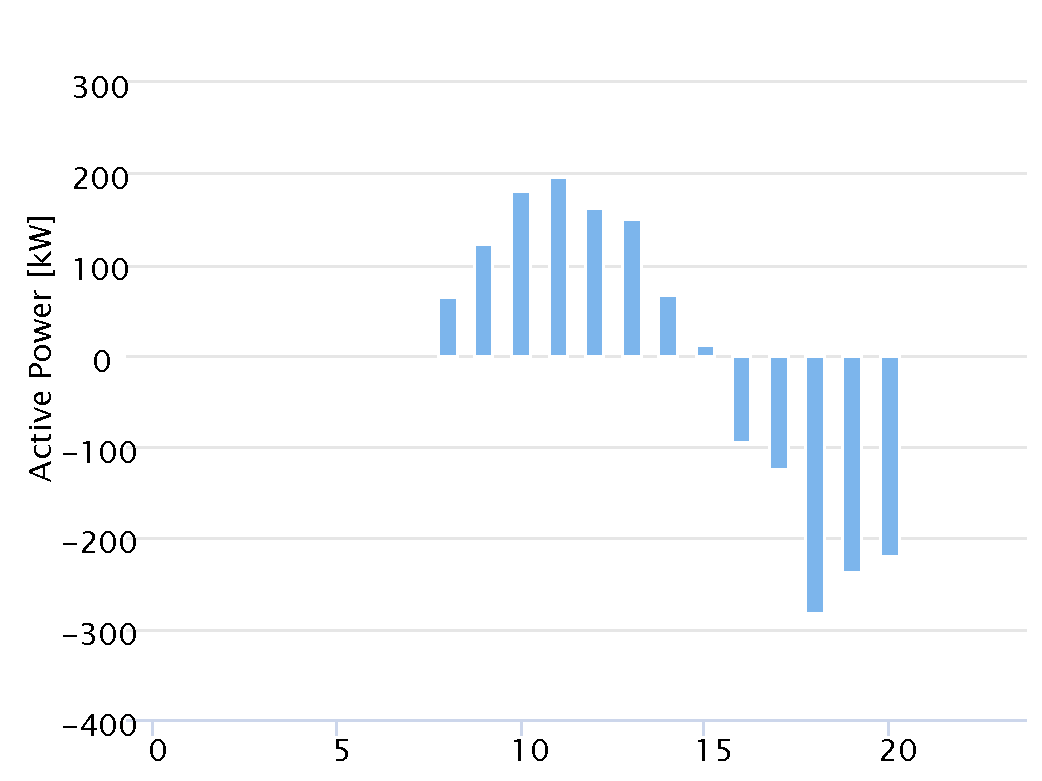
\includegraphics[height=0.8\textheight]{../Figures/7_case/bess-dispatch.pdf}
    \caption{BESS dispatch for case VI.}
\end{figure}
\end{frame}

\begin{frame}{Results: Case VII: Contingencies at 08:00 and 16:00 hours with EVs}
    \begin{columns}
    \begin{column}[c]{0.5\textwidth}
        \centering
        \begin{figure}
            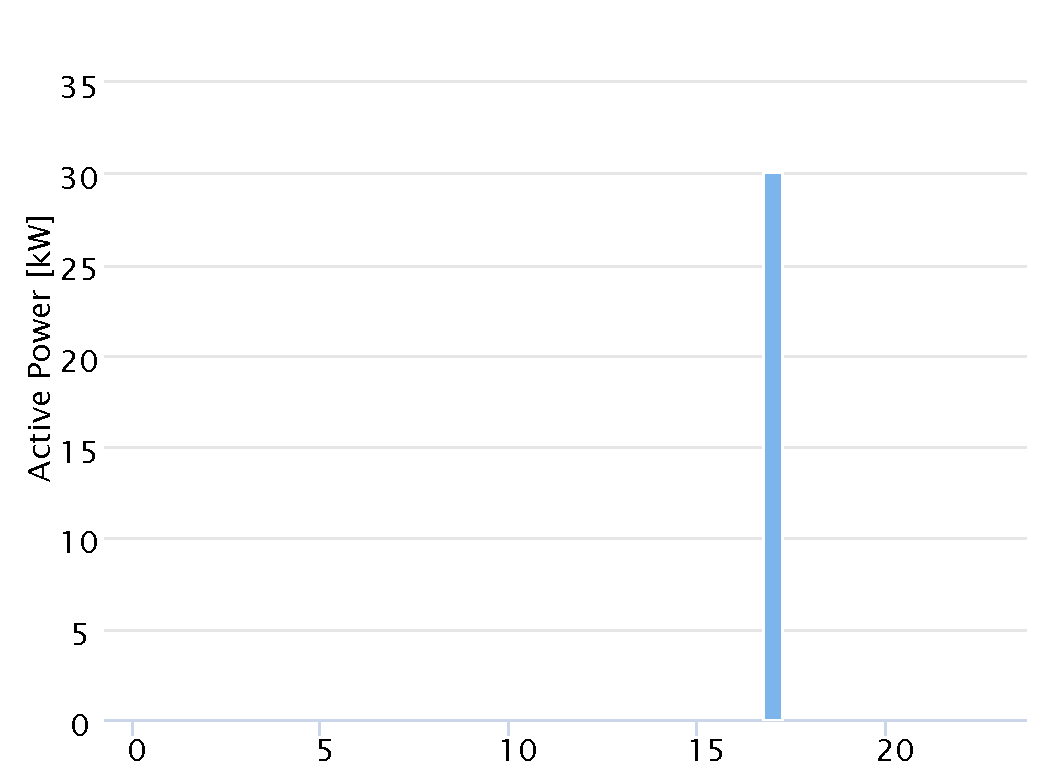
\includegraphics[height=0.65\textheight]
            {../Figures/7_case/genset-dispatch.pdf}
            \caption{Genset dispatch.}
        \end{figure}  
    \end{column}
    \begin{column}[c]{0.5\textwidth}
        \centering
        \begin{figure}
            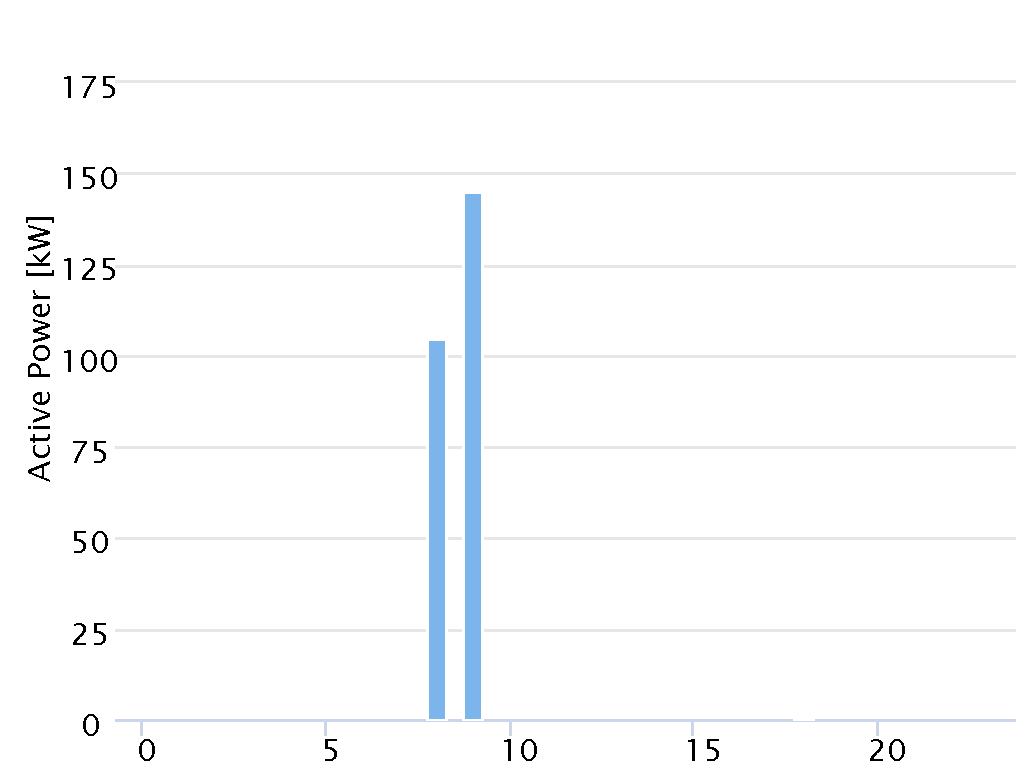
\includegraphics[height=0.65\textheight]
            {../Figures/7_case/pv-curtailment.pdf}
            \caption{PV curtailment.}
        \end{figure}  
    \end{column}
    \end{columns}
\end{frame}


\begin{frame}{Results: Case VII: Contingencies at 08:00 and 16:00 hours with EVs}
\begin{figure}
    \includegraphics[height=0.8\textheight]{../Figures/7_case/ev2.pdf}
    \caption{EV 2 dispatch.}
\end{figure}
\end{frame}


\begin{frame}{Results: Case VII: Contingencies at 08:00 and 16:00 hours with EVs}
\begin{figure}
    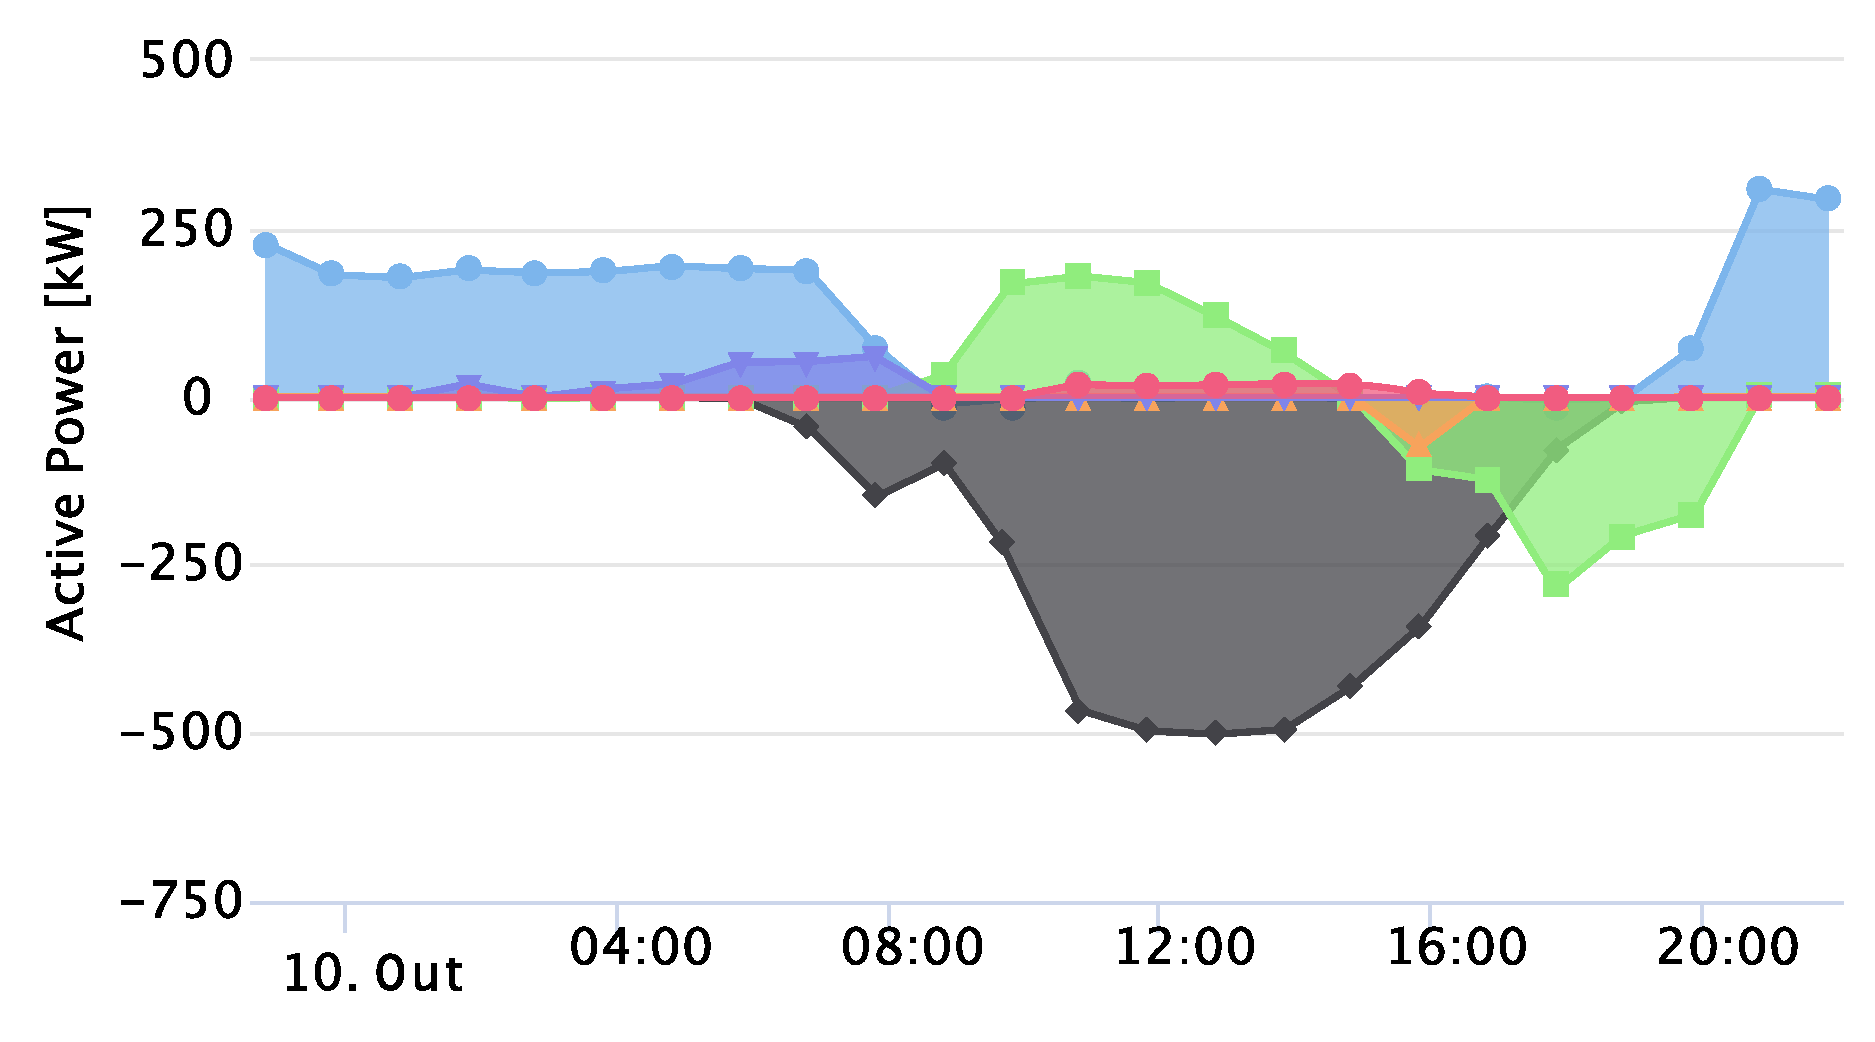
\includegraphics[height=0.8\textheight]{../Figures/7_case/microgrid-operation.pdf}
    \caption{Microgrid operation 24 hours.}
\end{figure}
\end{frame}



\section{Conclusions}

\begin{frame}
    \frametitle{Conclusions}

    \begin{itemize}[<+->]
        \item Developed a multi-objective optimization model for the EMS. 
        \item Integrated a new window of EVs in the IoT-based EMS.
        \item Validated the EMS in a Hardware-in-the-Loop (HIL) environment.
    \end{itemize}
\end{frame}

\begin{frame}{Work plan and schedule} 
    \begin{columns}
        \begin{column}[t]{0.6\textwidth}
            \begin{itemize} 
                \item \textbf{01:} Taking courses. 
                \item \textbf{02:} Continuing courses and introduction to the MERGE project. 
                \item \textbf{03:} Learning the CAMPUSGRID microgrid mathematical model using Python and Pyomo. 
                \item \textbf{04:} Implementing the mathematical model with linearizations, contingencies, and scenarios in Pyomo. 
                \item \textbf{05:} Gaining knowledge of backend (Flask API and database) and frontend (Angular) technologies. 
                \item \textbf{06:} Preparing case studies for 24-hour simulations with Typhoon HIL604 software. 
                \item \textbf{07:} Preparing for the qualification exam. 
                \item \textbf{08:} Continuing simulations, including a rolling horizon approach and PV forecasting. 
                \item \textbf{09:} Writing and preparing the master's thesis. 
                \item \textbf{10:} Defending the master's thesis. \end{itemize}        
        \end{column}
        \begin{column}[t]{0.5\textwidth}
            \begin{table}[]
                \caption{Scheduled and project status}
                \centering
                \label{tab:sche}
                \begin{tabular}{cllll}
                \textbf{Stage} &
                  \multicolumn{1}{c}{\textbf{\begin{tabular}[c]{@{}c@{}}1st\\ 2023\end{tabular}}} &
                  \multicolumn{1}{c}{\textbf{\begin{tabular}[c]{@{}c@{}}2nd\\ 2023\end{tabular}}} &
                  \multicolumn{1}{c}{\textbf{\begin{tabular}[c]{@{}c@{}}1st\\ 2024\end{tabular}}} &
                  \multicolumn{1}{c}{\textbf{\begin{tabular}[c]{@{}c@{}}2nd\\ 2024\end{tabular}}} \\ 
                  \hline
                \multicolumn{1}{|c|}{01} &
                  \multicolumn{1}{c|}{\cellcolor[HTML]{bdc6d1}} &
                  \multicolumn{1}{c|}{} &
                  \multicolumn{1}{c|}{} &
                  \multicolumn{1}{c|}{} \\ \hline
                \multicolumn{1}{|c|}{02} &
                  \multicolumn{1}{c|}{} &
                  \multicolumn{1}{c|}{\cellcolor[HTML]{bdc6d1}} &
                  \multicolumn{1}{c|}{} &
                  \multicolumn{1}{c|}{} \\ \hline
                \multicolumn{1}{|c|}{03} &
                  \multicolumn{1}{l|}{} &
                  \multicolumn{1}{c|}{\cellcolor[HTML]{bdc6d1}} &
                  \multicolumn{1}{c|}{} &
                  \multicolumn{1}{l|}{} \\ \hline
                \multicolumn{1}{|c|}{04} &
                  \multicolumn{1}{l|}{} &
                  \multicolumn{1}{l|}{\cellcolor[HTML]{bdc6d1}} &
                  \multicolumn{1}{c|}{} &
                  \multicolumn{1}{l|}{} \\ \hline
                \multicolumn{1}{|c|}{05} &
                  \multicolumn{1}{l|}{} &
                  \multicolumn{1}{l|}{} &
                  \multicolumn{1}{c|}{\cellcolor[HTML]{bdc6d1}} &
                  \multicolumn{1}{l|}{} \\ \hline
                \multicolumn{1}{|c|}{06} &
                  \multicolumn{1}{l|}{} &
                  \multicolumn{1}{l|}{} &
                  \multicolumn{1}{c|}{\cellcolor[HTML]{bdc6d1}} &
                  \multicolumn{1}{l|}{} \\ \hline
                \multicolumn{1}{|c|}{07} &
                  \multicolumn{1}{l|}{} &
                  \multicolumn{1}{l|}{} &
                  \multicolumn{1}{l|}{\cellcolor[HTML]{bdc6d1}} &
                  \multicolumn{1}{c|}{} \\ 
                  \hline
                \multicolumn{1}{|c|}{08} &
                  \multicolumn{1}{l|}{} &
                  \multicolumn{1}{l|}{} &
                  \multicolumn{1}{l|}{} &
                  \multicolumn{1}{c|}{\cellcolor[HTML]{ef233c}}\\ 
                  \hline
                \multicolumn{1}{|c|}{09} &
                  \multicolumn{1}{l|}{} &
                  \multicolumn{1}{l|}{} &
                  \multicolumn{1}{l|}{} &
                  \multicolumn{1}{l|}{\cellcolor[HTML]{ef233c}} \\ 
                  \hline
                \multicolumn{1}{|c|}{10} &
                  \multicolumn{1}{l|}{} &
                  \multicolumn{1}{l|}{} &
                  \multicolumn{1}{l|}{} &
                  \multicolumn{1}{l|}{\cellcolor[HTML]{ef233c}} \\ 
                  \hline
                &&&&\\
                 &
                  \multicolumn{2}{c}{\cellcolor[HTML]{bdc6d1}Done} &
                  \multicolumn{2}{c}{\cellcolor[HTML]{ef233c}To do}
                \end{tabular}
                \end{table}
        \end{column}
    \end{columns}
\end{frame}


\begin{frame}
    \begin{large}
        \begin{center}
            \textbf{Thank you!}
        \end{center}
    \end{large}

    \vspace{15pt}

    Acknowledgments:
    \vspace{-0.3cm}
    \begin{figure}
        \centering
        \includegraphics[width=\textwidth]{../Figures/agradecimentos.pdf}
    \end{figure}
\end{frame}
\end{document}
    